% Drawing 83/10-5 -- folder 83, batch 10, archive page 200 (PDF page 201).
% Transcription: troisième cube, arêtes étiquetées $\Sigma_1$, $\Sigma_2$, $\Sigma_3$.
% Kind: cube with labelled edges. Method 2 (schematic redraw from the facsimile). Status: ok.
% Notes: Third cube: Sigma_1 on the heavy left front edge, Sigma_2 on an inner diagonal stroke, Sigma_3 on an arrow under the bottom edge; the top right edge heavy (with a second label read as Sigma_2), the edge to the back top left dotted.
% Coordinates: 1 unit = 1 mm = 1/100 of the crop width (bbox in page fractions: [0.1, 0.66, 0.38, 0.82]).
% Redrawn by Claude (claude-opus-5-5), issue #73, 2026-11-07; not checked by a human; not compiled (no TeX in the session).
% Rights: reproduces part of the work -- behind RENDER_TRANSCRIPTS, never published by itself.
\documentclass[tikz,border=3pt]{standalone}
\usepackage{amsmath,amssymb}
\usetikzlibrary{patterns,arrows.meta}
\tikzset{pencil/.style={black!45}, struck/.style={black!35}, mark/.style={circle,draw,inner sep=1.3pt}, pt/.style={circle,fill,inner sep=0.9pt}, opt/.style={circle,draw,fill=white,inner sep=1.1pt}}
\begin{document}
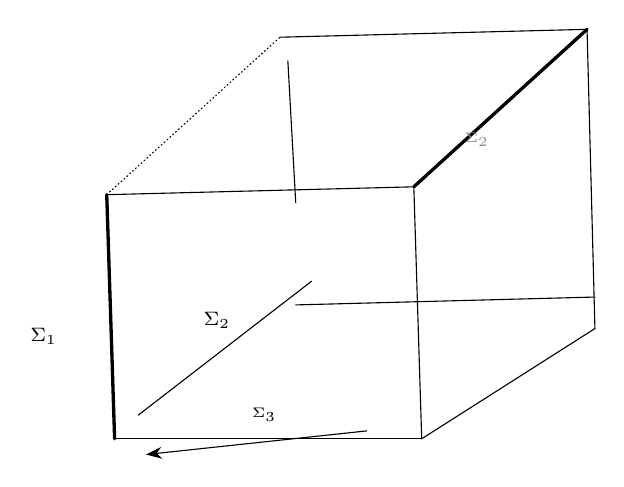
\begin{tikzpicture}[x=1mm,y=1mm,line cap=round,line join=round,font=\scriptsize]
\draw (36,-29) -- (75,-28);
\draw (75,-28) -- (76,-60);
\draw (76,-60) -- (37,-60);
\draw (58,-9) -- (97,-8);
\draw (97,-8) -- (98,-46);
\draw (76,-60) -- (98,-46);
\draw[very thick] (36,-29) -- (37,-60);
\draw[very thick] (75,-28) -- (97,-8);
\draw[densely dotted] (36,-29) -- (58,-9);
\draw (59,-12) -- (60,-30);
\draw (60,-43) -- (98,-42);
\draw (40,-57) -- (62,-40);
\draw[-{Stealth[length=2mm]}] (69,-59) -- (41,-62);
\node[inner sep=1pt] at (28,-47) {\scriptsize $\Sigma_1$};
\node[inner sep=1pt] at (50,-45) {\scriptsize $\Sigma_2$};
\node[inner sep=1pt] at (56,-57) {\tiny $\Sigma_3$};
\node[inner sep=1pt,pencil] at (83,-22) {\tiny $\Sigma_2$};
\end{tikzpicture}
\end{document}
